\documentclass[11pt,a4paper]{article}
\usepackage{amsmath,amssymb}
\usepackage{unicode-math}
\usepackage{lmodern}
\defaultfontfeatures{Ligatures=TeX}
\setmainfont[BoldFont=texgyrepagella-bold.otf,ItalicFont=texgyrepagella-italic.otf,BoldItalicFont=texgyrepagella-bolditalic.otf]{texgyrepagella-regular.otf}
\setmonofont[BoldFont=lmmonolt10-bold.otf]{lmmono10-regular.otf}
\setmathfont{texgyrepagella-math.otf}
\usepackage[margin=25mm,headheight=14pt,headsep=7mm]{geometry}
\usepackage{mathtools,booktabs,array,graphicx,xcolor,fancyhdr,needspace}
\usepackage[colorlinks=true,linkcolor=blue!40!black,citecolor=blue!40!black,urlcolor=blue!40!black]{hyperref}
\pagestyle{fancy}\fancyhf{}\lhead{\small Paired-gap geometry and observation}\rhead{\small Paper I: draft v0.1.1}\cfoot{\thepage}
\setlength{\parskip}{4pt}\setlength{\parindent}{1.2em}\setlength{\emergencystretch}{2em}\raggedbottom
\newtheorem{theorem}{Theorem}[section]
\newtheorem{proposition}[theorem]{Proposition}
\newtheorem{corollary}[theorem]{Corollary}
\newtheorem{definition}[theorem]{Definition}
\newtheorem{example}[theorem]{Example}
\newtheorem{remark}[theorem]{Remark}
\AddToHook{env/theorem/before}{\ifnum\value{section}=9\Needspace{18\baselineskip}\else\Needspace{8\baselineskip}\fi}
\AddToHook{env/proposition/before}{\Needspace{5\baselineskip}}
\AddToHook{cmd/subsection/before}{\Needspace{8\baselineskip}}
\AddToHook{cmd/section/before}{\Needspace{12\baselineskip}}
\newenvironment{proof}{\par\noindent\textit{Proof.}\ }{\hfill$\square$\par}
\newcommand{\R}{\mathbb R}\newcommand{\C}{\mathbb C}\newcommand{\ez}{e_z}
\newcommand{\diag}{\operatorname{diag}}\newcommand{\rank}{\operatorname{rank}}
\newcommand{\dist}{\operatorname{dist}}\newcommand{\conv}{\operatorname{conv}}
\newcommand{\Id}{\mathbf I}\newcommand{\Ch}{\mathcal C}\newcommand{\norm}[1]{\lVert#1\rVert}
\newcommand{\tr}{^{\mathrm T}}\newcommand{\kk}{K_0}
\hypersetup{pdftitle={Paired-Gap Geometry and Toroidal Observation Maps for the Folded Tri-Octagon},pdfauthor={Hilmir Frimann Halldorsson},pdfsubject={Paper I; draft v0.1.1}}
\begin{document}
\begin{center}
{\LARGE\bfseries Paired-Gap Geometry and\par Toroidal Observation Maps\par for the Folded Tri-Octagon\par}
\vspace{5mm}
{\large Hilmir Fr\'imann Halld\'orsson}\par
\vspace{3mm}18 October 2026\quad Paper I\quad Draft v0.1.1
\end{center}
\begin{abstract}
We study three paired upper/lower measurement regions of the width-one folded Tri-Octagon and complete quarter-turned reference modules placed around it. The material shell is the annulus established in Paper C; the toroidal constructions are additional geometry. Within a stated median circular family, normal crossing of a pair fixes a unique circle, with exact interior contacts and clearance from every filled panel. The six contacts cannot belong to one planar circle. A conditional uniform observation map resolves a registered three-vector from twelve frames, while its staged native-state records have generic real rank four rather than six. A second, explicitly conditional interface introduces six Euclidean delays. We prove a weighted transfer bound, a controlled differential-delay expansion, height/reflection identities, and an all-frequency inverse at aligned equatorial sites. A pure-delay tangential component and an off-ring blind-frequency example distinguish geometry from interference. Contact-onset and storage calculations show precisely why this comparator supplies neither imposed field boundary values nor a finite physical source-energy budget. Full proofs, source distinctions and static coordinate figures connect the author's paired-loop and multi-ring questions to these limited but explicit observation models.
\end{abstract}
\tableofcontents

\section{The geometric question and the mathematical objects}\label{sec:intro}
This study was motivated by Hilmir Fr\'imann Halld\'orsson's proposal to examine paired upper and lower regions of the folded Tri-Octagon, a transverse local loop, and twelve smaller, quarter-turned copies of the complete module arranged around the centre. We ask which geometric relationships and observation signatures follow once the shell, registration and measurement rules are specified explicitly. The three upper/lower pairs are labelled $P0,P1,P2$.~\cite{AuthorPair,AuthorScope}

The multi-ring proposal compares observers at higher and lower levels, observers farther outward, and a possible combination. Earlier reception is a motivating hypothesis: height, radius and reception time cannot be equated before a reception rule has been supplied. We therefore treat the five-height and three-radius arrangements as controlled comparisons, with the broader combined arrangement left symbolic. The numerical dimensions used below are the declared comparison choices of SRG-04.~\cite{AuthorMulti,SRG04}

Four kinds of object must remain distinct. First, the shell is a fixed subset of Euclidean three-space, defined by filled polygons. Second, the native state is a complex triad with its separately specified recurrence and readouts. Third, a geometric registration sends ordered readout data into a chosen measurement frame. Fourth, an observation law specifies what the reference modules record. Neither the shell alone nor a drawing supplies the third and fourth objects. This separation allows a positive geometric result and an information obstruction to coexist without changing the original kernel.

Paper C fixes the welded shell, its width normalization and its topology.~\cite[Secs.~2--5]{PC} The Gate/Torus source specifies the complete quarter-turned placement.~\cite[Sec.~6]{Gate} SRG-02 selects a conditional normal-crossing local circle; SRG-03 adds the uniform observation convention; SRG-04 adds the delay-only comparator.~\cite{SRG02,SRG03,SRG04} The distinction between a reconstructed field and imposed field boundary data is retained throughout, as in the accompanying internal reviews.~\cite{Reviews}

The geometric-origins companion places these questions within the earlier normalization study and sustained human--AI collaboration.~\cite[Secs.~1--3]{Origins} Possible applications to computation remain a motivation; software performance and nonlinear encoding are subjects of a later paper.

\subsection{Notation and units}\label{sec:notation}
All geometric lengths below are in units of the panel flat-to-flat width. Multiplying every coordinate and length by a chosen $w>0$ restores a dimensional length unit; the numerical reference is $w=1$. This does not set a physical length scale.

\begin{table}[htbp]\centering\small
\caption{Object dictionary. Distinct symbols prevent inherited notational collisions.}
\begin{tabular}{@{}p{40mm}p{113mm}@{}}\toprule
Symbol & Meaning and convention\\\midrule
$w=1$, $s=\sqrt2-1$ & Panel width and panel edge length, respectively.\\
$O$, $B_j$ & Shell centre and centre of a selected local circle.\\
$a$, $R_\Gamma$, $R_m$ & Median contact offset, local-circle radius, observer placement radius. $a$ is not Paper C's octagon apothem $w/2$.\\
$\kk$, $\mathbf K(X,\omega)$ & Patch-plane constant (called $K$ in SRG-02) and delay transfer matrix (called $K$ in SRG-04).\\
$\Ch=x\times y$ & Channel chirality, called $C$ in the native/readout sources. It is not a circle centre, a circumference, or the suffix in Paper C.\\
$s_m$, $c_*$ & Dimensionless miniature scale and declared delay speed (width units per analysis-time unit).\\
$n$, $(q,N,t_c)$ & Native iteration and independently supplied readout-clock state.\\
$t$, $k$, $\chi$ & Analysis time, spatial observer index, and local-circle angle. None is identified with the other two.\\
$A$, $W_v$ & Fixed conditional registration and its virtual polar measurement vector for ordered triple $v$.\\
$E$ & Model-defined delay-line storage; units are signal squared times length.\\\bottomrule
\end{tabular}\label{tab:notation}
\end{table}

\section{The fixed shell and its three paired regions}\label{sec:shell}
\subsection{An exact coordinate realization}
Put $s=\sqrt2-1$, $d=1-\sqrt2/2$, $h_0=s/2$. In a panel's coordinates $(u,z)$ use the cyclic list
\begin{equation}\label{eq:octagon}
\begin{split}
(-\tfrac12,-h_0),\ (-h_0,-\tfrac12),\ (h_0,-\tfrac12),\ (\tfrac12,-h_0),\\
(\tfrac12,h_0),\ (h_0,\tfrac12),\ (-h_0,\tfrac12),\ (-\tfrac12,h_0).
\end{split}
\end{equation}
Let $D_8$ be their filled convex octagon. The three isometric embeddings are
\begin{equation}\label{eq:panels}
\begin{aligned}
f_1(u,z)&=(-\tfrac14-\tfrac u2,\ \tfrac{\sqrt3}4-\tfrac{\sqrt3}2u,\ z),\\
f_2(u,z)&=(u,0,z),\\
f_3(u,z)&=(\tfrac14-\tfrac u2,\ \tfrac{\sqrt3}4+\tfrac{\sqrt3}2u,\ z).
\end{aligned}
\end{equation}
The material shell is $S=f_1(D_8)\cup f_2(D_8)\cup f_3(D_8)$, with centre $O=(0,\sqrt3/6,0)$. Thus $S$ includes the entire panels, not only their edges. Equations \eqref{eq:octagon}--\eqref{eq:panels} reproduce Paper C's width-one realization without any project import.~\cite[Secs.~2--4]{PC}

The welded vertex numbering is fixed as follows. Traverse $f_1$ in the order \eqref{eq:octagon} and assign IDs $0,\ldots,7$. The $f_2$ cycle is $(3,8,9,10,11,12,13,4)$; the $f_3$ cycle is $(10,14,15,0,7,16,17,11)$. This is a complete coordinate prescription for all eighteen vertices, including each alias at a seam. The three seams are $(0,7),(3,4),(10,11)$.

\begin{proposition}[Inherited shell topology]\label{prop:topology}
The specified shell is a connected compact orientable surface with boundary, with eighteen vertices, twenty-one edges, three faces and two disjoint nine-edge boundary rims. It is an annulus.
\end{proposition}
\begin{proof}
We reuse Paper C, Section 5, Theorems 1 and 1b, with exactly the maps \eqref{eq:panels}. To make the inherited hypotheses visible: the three seams identify three pairs of edges and six pairs of vertices, giving $E=24-3=21$ and $V=24-6=18$. The face adjacency graph is connected. Each seam interior has two glued half-disc neighbourhoods; each free edge has one. Every vertex link is an interval: a single-panel corner gives one link edge, and a seam endpoint gives two joined link edges. The panel planes meet only along the prescribed seams within the panels. Opposite traversal of each seam by its adjacent face cycles gives orientation. Tracing the eighteen free edges gives one nine-edge cycle above $z=0$ and another below it. Consequently $\chi=18-21+3=0$ and $b=2$. The orientable-surface classification applied in the cited theorem gives $0=2-2g-2$, hence genus zero and the annulus type. A torus would instead have no boundary.
\end{proof}

\subsection{Finite measurement triangles}
Define
\begin{equation}\label{eq:axes}
r_0=1/\sqrt3,\quad c=\sqrt3/2,\quad
u_j=R_z(2\pi j/3)(0,1,0),\quad v_j=\ez\times u_j,
\end{equation}
where $j=0,1,2$ and $R_z$ is the ordinary right-handed rotation. The three seam footprints are $O+r_0u_j$. For $\sigma\in\{+1,-1\}$ set
\begin{equation}\label{eq:triangles}
\Delta_j^\sigma=\left\{O+(r_0-cdt)u_j+\xi v_j+\sigma(h_0+dt)\ez:
0\le t\le1,\ |\xi|\le dt/2\right\}.
\end{equation}
Here $t$ is a triangle coordinate only; analysis time will occur only in later sections. The two tip-to-base sides are material rim edges. The third side closes a measurement region between the two base vertices and adds no material panel or cap. The orientation and ID order are
\begin{center}
\begin{tabular}{@{}ccc@{}}\toprule
Pair & Upper, tip first & Lower, tip first\\\midrule
$P0$ & $(7,6,16)$ & $(0,15,1)$\\
$P1$ & $(4,13,5)$ & $(3,2,8)$\\
$P2$ & $(11,17,12)$ & $(10,9,14)$\\\bottomrule
\end{tabular}
\end{center}
These triangles describe three paired geometric regions, not six additional boundary components. In particular, their shared upper/lower projected footprints are not an identification of their spatial points.

\begin{proposition}[Planes, normals and contacts]\label{prop:contacts}
The oriented unit normals and supporting planes of \eqref{eq:triangles} are
\begin{equation}\label{eq:planes}
n_j^\sigma=\frac{2u_j+\sigma\sqrt3\ez}{\sqrt7},\qquad
u_j\cdot(X-O)+\sigma cX_z=\kk,\quad
\kk=\frac{\sqrt3}{12}+\frac{\sqrt6}{4}.
\end{equation}
Let $a=\kk/(1+c)$. The selected median points
\begin{equation}\label{eq:contacts}
P_j^\pm=O+a u_j\pm a\ez,\qquad t_0=(a-h_0)/d
\end{equation}
belong to the relative interiors of their triangles, with tip-first barycentric coordinates $(1-t_0,t_0/2,t_0/2)$.
\end{proposition}
\begin{proof}
Substitution in the left side of \eqref{eq:planes} gives $r_0-cdt+c(h_0+dt)=r_0+ch_0=\kk$. The two tangent directions $v_j$ and $-c u_j+\sigma\ez$ are perpendicular to the stated unit normal; the printed vertex orders give its sign. At $P_j^\sigma$, the plane equation is $a(1+c)=\kk$ and the transverse coordinate is zero. Also
\[
a-h_0=\frac{r_0-h_0}{1+c}>0,\qquad
\tfrac12-a=\frac{(1+c)/2-\kk}{1+c}>0.
\]
For explicit inequalities, $h_0<1/4<r_0$ follows from $\sqrt2<3/2$ and $\sqrt3<2$; and $(1+c)/2-\kk=1/2+\sqrt3/6-\sqrt6/4>0$, since $\sqrt3>3/2$ and $\sqrt6<5/2$ give a lower bound $1/8$. Since $h_0+d=1/2$, we have $0<t_0<1$. The triangle is the affine interpolation between its tip and its base segment, so the displayed barycentrics follow and are strictly positive.
\end{proof}

Numerically, $\kk\simeq0.756710$, $a\simeq0.405520$, and $t_0\simeq0.677424$. These values are consequences of the specified planes. The contacts are not triangle centroids. Their selection is the median member of the recovered Gate/Torus contact family, not a fit to any unrelated constant.~\cite[Sec.~3.3]{Gate}

\section{A conditional normal-crossing circle}\label{sec:circle}
We now make the added geometric choice explicit: seek a Euclidean circle in the affine median plane $O+\operatorname{span}(u_j,\ez)$, through $P_j^+$ and $P_j^-$, with tangent parallel to the relevant patch normal at each contact. This is one precise version of the transverse-loop picture. Its uniqueness is relative to this family.

\begin{theorem}[Selected circle and finite crossings]\label{thm:circle}
There is exactly one circle with those properties. Its centre, radius and oriented parametrization are
\begin{equation}\label{eq:circle}
B_j=O+\kk u_j,\quad R_\Gamma=\frac{\sqrt7}2a,\quad
\Gamma_j(\chi)=B_j+R_\Gamma(\cos\chi\,u_j+\sin\chi\,\ez).
\end{equation}
It meets each of its two finite measurement triangles exactly once, at $P_j^\sigma$, with unit tangents $-n_j^+$ above and $+n_j^-$ below. It meets none of the other four triangles.
\end{theorem}
\begin{proof}
Equal distances from a planar centre $O+b u_j+z_b\ez$ to $P_j^+$ and $P_j^-$ give $4az_b=0$, hence $z_b=0$. Orthogonality of the upper contact radius to the prescribed normal then requires
\[
0=(P_j^+-B_j)\cdot n_j^+
=\frac{2(a-b)+\sqrt3a}{\sqrt7}.
\]
Thus $b=(1+c)a=\kk$ and the radius squared is $(a-\kk)^2+a^2=(1+c^2)a^2=7a^2/4$. The lower condition gives the same equation. These deductions are necessary and, by substitution, sufficient, proving uniqueness.

At the contacts, $\cos\chi=-\sqrt{3/7}$ and $\sin\chi=\sigma2/\sqrt7$. Differentiating \eqref{eq:circle} gives the stated unit tangents. The supporting plane cuts the circle in a line through $B_j$ because $u_j\cdot(B_j-O)=\kk$. Its two intersections are therefore $P_j^\sigma$ and $2B_j-P_j^\sigma$. The latter has height $-\sigma a$, whereas every point of $\Delta_j^\sigma$ has height of sign $\sigma$. Only the first intersection belongs to the finite triangle. Proposition~\ref{prop:contacts} proves its interior membership, and the nonzero normal derivative proves transversality.

For $\ell\ne j$, a point of $\Delta_\ell^\sigma$ has $u_j$ projection at most
\[
-\tfrac12(r_0-cdt)+\tfrac{\sqrt3}{2}\tfrac{dt}{2}
=-r_0/2+cdt\le-r_0/2+cd<0.
\]
The last inequality is $d<1/3$, which follows from $\sqrt2>4/3$. The circle's projection is at least $\kk-R_\Gamma>0$, because $1+c>\sqrt7/2$. It cannot reach another pair.
\end{proof}

The right-angle operation has a definite pivot and order. Start with the horizontal parent circle $B_j+R_\Gamma(\cos\chi\,u_j+\sin\chi\,v_j)$ and rotate by $+\pi/2$ about the radial line through $O$ and $B_j$, using $B_j$ as pivot. This sends $v_j$ to $\ez$ and $\ez$ to $-v_j$. The resulting circle's axis is $-v_j$, perpendicular to the central shell axis. The shell itself is not rotated by this operation.

\begin{theorem}[Whole-circle clearance and the planar obstruction]\label{thm:clearance}
Each $\Gamma_j$ is disjoint from the filled shell $S$. The three circles are mutually disjoint, with pairwise distance at least $\sqrt3(\kk-R_\Gamma)>0$. No plane, hence no planar circle, contains all six selected contacts.
\end{theorem}
\begin{proof}
Work in a fixed median plane and write $X-O=r u_j+z\ez$. The opposite panel has meridian section $r=-1/(2\sqrt3)$. Since $r\ge\kk-R_\Gamma>0$ on the circle, that panel is excluded. The remaining two panel planes meet this median plane only on their common seam line $r=r_0$; their material portions there satisfy $|z|\le h_0$. The circle instead has, at that line,
\begin{equation}\label{eq:seamclear}
z^2=R_\Gamma^2-(r_0-\kk)^2
=\frac{113}{6}+\frac{13\sqrt2}{2}-\frac{133\sqrt3}{12}-\frac{7\sqrt6}{2}>\frac14>h_0^2.
\end{equation}
For a fully explicit certificate of the close first inequality, use the rational enclosures
\[
\begin{array}{c}
1.41421356237<\sqrt2<1.41421356238,\\
1.73205080756<\sqrt3<1.73205080757,\\
2.44948974278<\sqrt6<2.44948974279.
\end{array}
\]
Each follows by squaring positive rational endpoints. Substitution of lower endpoints in positive terms and upper endpoints in negative terms gives a rational lower bound greater than $0.2556109383$, itself greater than $1/4$. The second inequality follows from $h_0<1/4$. This covers panel interiors as well as edges, without sampling the circle.

For two different median planes, points of the circles have horizontal projections $r u_j$ and $r' u_\ell$, with $r,r'\ge m:=\kk-R_\Gamma>0$. Since $u_j\cdot u_\ell=-1/2$, their squared horizontal distance is $r^2+r'^2+rr'\ge3m^2$. Vertical differences only increase total distance. Finally, the three upper contacts form a nondegenerate triangle in $z=a$; they determine that plane. No lower contact with $z=-a$ lies in it. This proves the planar obstruction.
\end{proof}

\begin{figure}[htbp]\centering
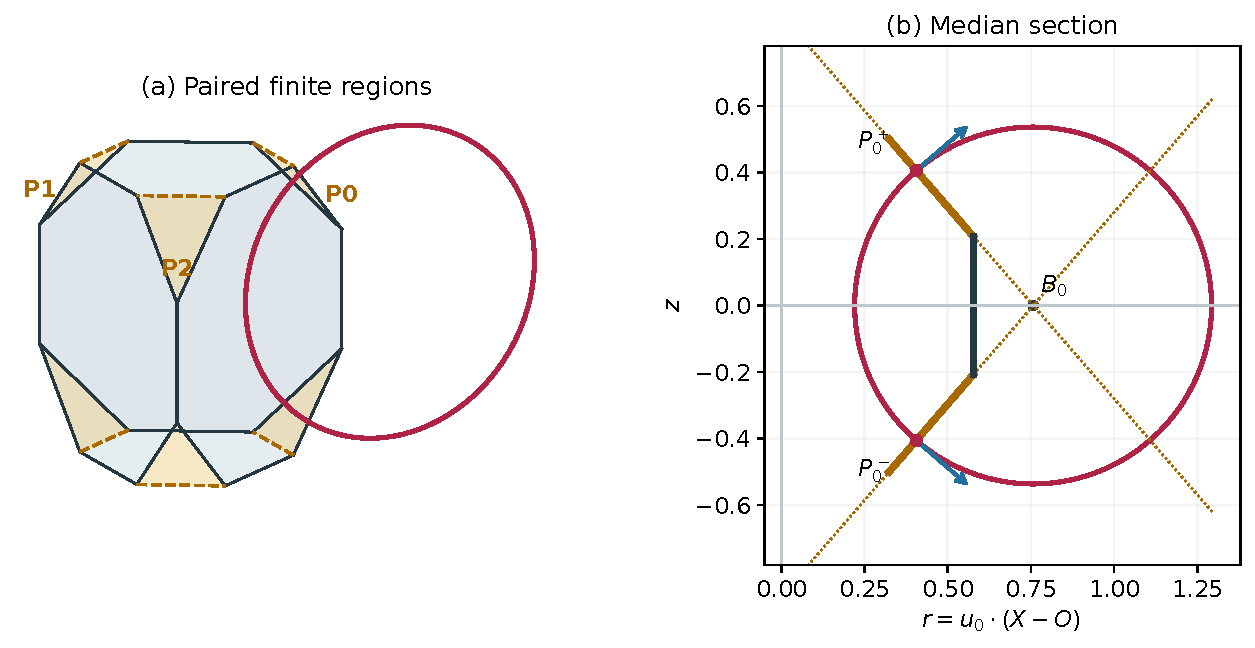
\includegraphics[width=\linewidth]{figures/paired_geometry.pdf}
\caption{Width-one paired geometry and the selected local circle. Left: all material panels and edges, with three upper/lower measurement pairs; dashed gold bases are measurement-only closures. Only $\Gamma_0$ is drawn. Right: its median section, exact interior contacts and patch normals. The blue vectors are geometric normals. The finite measurement segments are distinguished from their dotted supporting lines. Red is a spatial centreline without a time or flow law.}\label{fig:geometry}
\end{figure}

\subsection{A shared point does not establish a shared path}\label{sec:grazing}
The recovered unit frozen macro reference has, near an upper median contact, the curve
\begin{equation}\label{eq:macrocurve}
\mathcal M_j(\nu)=O+a\cos3\nu(\cos\nu\,u_j+\sin\nu\,v_j+\ez).
\end{equation}
At $\nu=0$ it equals $P_j^+$, but $\mathcal M_j'(0)=a v_j$. Its signed plane residual is
\[
f(\nu)=a\cos3\nu(\cos\nu+c)-\kk,\qquad
f(0)=f'(0)=0,\quad f''(0)=-a(10+9c)<0.
\]
Thus it grazes that plane locally, whereas Theorem~\ref{thm:circle} gives a normal crossing. In fact $f\le0$ globally, with equality only at $\nu\in2\pi\mathbb Z$: the product is at most $|\cos\nu+c|\le1+c$, and the latter bound is attained only when $\cos\nu=1$. The other two extrema concern rotated patches, not additional equality points for this fixed patch. This incorporates the later direction-note qualification to the original contact review.~\cite[Sec.~5.4]{GateDirections}

The reference amplitude in \eqref{eq:macrocurve} is a geometric calibration. It is not a supplied native record. For example, the literal staged defaults and $t_c\ge0$ below give $|z_s|\le0.618$; the fixed median scale $a$ would require unit reference amplitude to reach a selected median contact. The construction does not claim that an observed staged point has passed through a patch. Also $M(-z_s)=-M(z_s)$ reverses the horizontal ray as well as height; it is not merely an upper/lower relabelling of a fixed pair.~\cite[Sec.~5.1]{GateDirections}

\subsection{What a tube would add}
One may write the optional family
\begin{equation}\label{eq:tube}
T_j(\chi,\psi;\tau)=B_j+(R_\Gamma+\tau\cos\psi)
(\cos\chi\,u_j+\sin\chi\,\ez)+\tau\sin\psi\,v_j.
\end{equation}
For $0<\tau<R_\Gamma$, the two parameter derivatives are perpendicular with nonzero lengths $R_\Gamma+\tau\cos\psi$ and $\tau$, so this is a regular circular torus. The positive radial factor also gives the usual embedded torus, rather than a spindle self-intersection. Compactness and Theorem~\ref{thm:clearance} imply $\dist(\Gamma_j,S)>0$. The additional sufficient condition $\tau<\dist(\Gamma_j,S)$ makes the tube disjoint from $S$, by the triangle inequality. No numerical thickness or minimum clearance is chosen here. Likewise three possible circles do not choose a physical loop count. A common carrier through all six contacts would require a separately defined nonplanar geometry.

\section{Complete quarter-turned observer modules}\label{sec:placement}
Let $e_r(\phi)=(\cos\phi,\sin\phi,0)$ and $e_\phi(\phi)=(-\sin\phi,\cos\phi,0)$. The recovered Gate/Torus operation is a composition, not just a rotation matrix. First centre a point of the complete shell, then apply
\begin{equation}\label{eq:frames}
Q_x(\pi/2)=\begin{pmatrix}1&0&0\\0&0&-1\\0&1&0\end{pmatrix},\qquad
B(\phi)=[e_r,e_\phi,\ez]Q_x(\pi/2)=[e_r,\ez,-e_\phi].
\end{equation}
Scale the result by $s_m>0$ and translate it to a specified centre. In the original shell coordinates the general ring is
\begin{equation}\label{eq:placement}
\begin{aligned}
\phi_{mk}&=\phi_{m0}+2\pi k/12,& k&=0,\ldots,11,\\
c_{mk}&=O+R_m e_r(\phi_{mk})+h_m\ez,& R_m&>0,\\
X_{mk}(p)&=c_{mk}+s_m B(\phi_{mk})(p-O),&p&\in S.
\end{aligned}
\end{equation}
The local first axis before the moving frame is the quarter-turn axis. Thus $B\ez=-e_\phi$, while $B$ is right-handed orthonormal. Each object is all three filled panels of $S$. Neither a point marker nor a sphere replaces the object; a bounding sphere below is only a clearance tool. The original Gate coordinates put the common centre at zero; adding $O$ in \eqref{eq:placement} expresses the same construction in Paper C coordinates.~\cite[Sec.~6]{Gate}

\begin{proposition}[Sufficient full-module clearances]\label{prop:balls}
Put
\[
B_S=\sqrt{13/12-\sqrt2/2},\qquad \rho_m=s_mB_S.
\]
Within one ring, between two distinct rings, and from each ring to the central shell and every local circle, respectively, sufficient separation conditions are
\begin{equation}\label{eq:bounds}
\begin{aligned}
2R_m\sin(\pi/12)&>2\rho_m,\\
\sqrt{(R_m-R_n)^2+(h_m-h_n)^2}&>\rho_m+\rho_n,\\
\sqrt{R_m^2+h_m^2}&>B_S+\rho_m,\\
\sqrt{R_m^2+h_m^2}&>\kk+R_\Gamma+\rho_m.
\end{aligned}
\end{equation}
These bounds concern filled modules and do not depend on their orientations.
\end{proposition}
\begin{proof}
The panel-centre distance from $O$ is $1/(2\sqrt3)$; the local vertex radius squared is $1/4+h_0^2$. Their perpendicular sum is $B_S^2$. All vertices thus lie in the radius-$B_S$ ball, and convexity places each entire polygon in that ball. A scaled, orthogonally placed copy lies in the radius-$\rho_m$ ball about its centre. On a twelve-site ring, the smallest centre distance is the adjacent chord $2R_m\sin(\pi/12)$. Between rings it is at least the second left side of \eqref{eq:bounds}, because the squared horizontal distance is $(R_m-R_n)^2+2R_mR_n(1-\cos\Delta\phi)$. The shell and each circle are contained in balls about $O$ of radii $B_S$ and $\kk+R_\Gamma$. Subtracting the two enclosing radii from a centre distance proves every claim. The bound is sufficient, not an optimized packing or exact surface distance.
\end{proof}

The H family has five levels $h_2,h_1,0,-h_1,-h_2$, with $0<h_1<h_2$ and freely declared radii, scales and angular origins. The R family has three ordered radii $R_1<R_2<R_3$ at a common height. For the accepted controls, H fixes $R_m=3$, $s_m=1/4$, $h_m\in\{2a,a,0,-a,-2a\}$; R fixes $h_m=0$, $s_m=1/4$, $R_m\in\{2,3,4\}$. Both use $\phi_{m0}=\pi/2$. All bounds in \eqref{eq:bounds} are positive; the smallest fixture margin is $a-B_S/2=0.0988331215\ldots$. These are separate controls. Their 60 and 36 labels total 96, but H0 and the middle R ring are the same twelve sites and frames. Their union has 84 distinct sites. It is not an instantiated height-by-radius product. The combined family remains the parameter list $(R_{\ell r},h_\ell,s_{\ell r},\phi_{\ell r,0})$.

\begin{proposition}[Matched centres are not mirrored bodies]\label{prop:mirror}
For equal radius, scale and angular origin at heights $\pm h$, horizontal reflection interchanges the centres and enclosing balls. Under the same-$B$ convention in \eqref{eq:placement}, it does not interchange the complete miniature shells.
\end{proposition}
\begin{proof}
Let $S_z=\diag(1,1,-1)$. Then $S_zB=B D$, where $D=\diag(1,-1,1)$ acts in the centred source coordinates. Literal reflection of a complete module would therefore require $D(S-O)=S-O$. A seam vertex has centred local $y=\sqrt3/3$; its $D$ image has $y=-\sqrt3/3$, below the minimum centred $y=-\sqrt3/6$ of $S$. Thus this equality fails. The centres and balls still reflect, because the centre heights change sign and a ball is invariant under all orthogonal maps.
\end{proof}

\begin{figure}[htbp]\centering
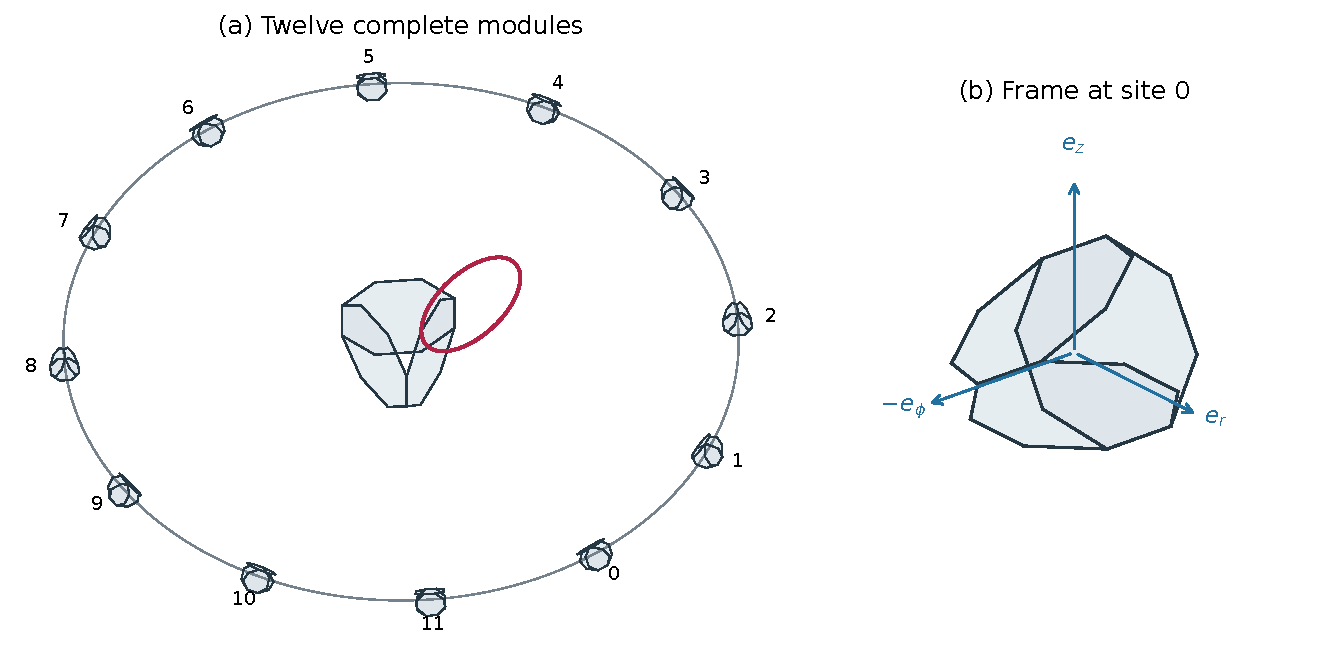
\includegraphics[width=\linewidth]{figures/full_modules.pdf}
\caption{Recovered full-module placement, with $R_c=3$, $s_k=1/4$, $\phi_0=0$. All twelve complete shells are drawn. The inset shows the local orthonormal frame and the original shell axis carried to $-e_\phi$. Grey is the exterior placement circle; red is the separate local $\Gamma_0$. No connecting surface is implied.}\label{fig:modules}
\end{figure}

\begin{figure}[htbp]\centering
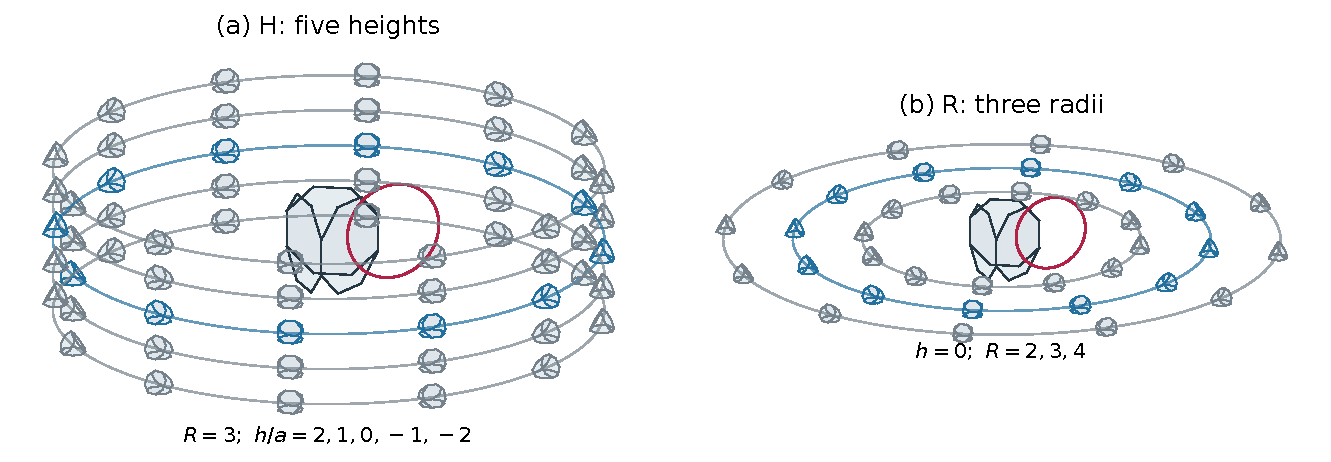
\includegraphics[width=\linewidth]{figures/hr_controls.pdf}
\caption{Separate H and R controls with their prescribed complete modules ($s_m=1/4$, $\phi_{m0}=\pi/2$). H varies height at radius 3; R varies radius at height zero. The common H0/R2 ring is highlighted in blue. Height matching reflects centres and bounding balls, not complete bodies under the same-$B$ convention. No H$\times$R layout is evaluated.}\label{fig:hr}
\end{figure}

% Flush geometry floats before the native-update section; mathematical sources remain unchanged.
\clearpage
\section{Native readouts and a typed uniform observation map}\label{sec:uniform}
\subsection{State, clock and geometric registration}
Write the native state as $\Omega=x+iy\in\C^3$, with $x,y\in\R^3$. The sourced recurrence first forms
\begin{equation}\label{eq:native}
\widetilde\Omega_i=\Omega_i+\epsilon\Omega_i(k_i-|\Omega_i|^2)
+g(L_3\Omega)_i,\qquad
L_3=\begin{pmatrix}-2&1&1\\1&-2&1\\1&1&-2\end{pmatrix},
\end{equation}
then synchronizes phases simultaneously. If $\vartheta_i=\operatorname{Arg}_0\widetilde\Omega_i$, with $\operatorname{Arg}_0(0)=0$, its mathematical expression is
\begin{equation}\label{eq:sync}
\Omega_i^+=|\widetilde\Omega_i|\exp\!\left(i\left[\vartheta_i+\lambda_s
\sum_{j\ne i}\sin3(\vartheta_j-\vartheta_i)\right]\right).
\end{equation}
Exact zero components remain zero. The source's zero-strength branch returns the pre-sync state directly. These formulas identify the native object; we do not execute it or assert a physical time step. The shell, receiver positions and observation laws below are not arguments of the recurrence.~\cite{Native}

The separate face decoder assigns $D_i(\Omega_i)=x_i t_i+y_i\ez$ to the tangent plane of face $i$, with its sourced horizontal unit tangent $t_i$. This is a triple of face-attached vectors, not a single ambient vector at all exterior sites. Its area triple is the channel-indexed cross product below; the distinction motivates the explicit dictionary rather than an implicit conversion to a spatial field.~\cite{Native}

The staged readout uses a supplied clock $(q,N,t_c)$, where $q$ is integer, $N$ is a positive integer and $t_c$ is an independent scalar. Define
\begin{equation}\label{eq:staged}
\begin{aligned}
\kappa&=\norm{\Omega},& I&=\kappa^2,&\Ch&=x\times y,\\
\theta&=2\pi(q\bmod N)/N,&
b&=\lambda_{vp}e^{-\gamma t_c}\cos3(\theta-\ell),\\
z_s&=b\frac{\kappa}{1+\kappa},&
M&=z_s(\cos\theta,\sin\theta,1),&T&=\alpha M+\beta\Ch.
\end{aligned}
\end{equation}
The literal defaults are $(\lambda_{vp},\gamma,\ell,\alpha,\beta)=(0.618,0.577,0.244,1,0.5)$. We write $z_s$ for the sources' scalar $z$, avoiding confusion with a spatial coordinate. The observer index $k$ does not replace $q$. A changed clock can change $M$ at fixed $\Omega$, without any motion of an observer or native evolution.~\cite{Readout}

\begin{definition}[Conditional virtual dictionary]\label{def:dictionary}
Fix, before comparing states, $A=\lambda_gR_z(\delta)$ with $\lambda_g>0$. For each ordered readout triple $v\in\{M,\Ch,T\}$, define $W_v=Av$ as a virtual polar measurement vector. For a complete observer frame, a paired normal, and a circle tangent respectively, record
\begin{equation}\label{eq:uniform}
\begin{aligned}
y_k^v&=B_k\tr W_v,\qquad \mathcal R_k=(z_s,y_k^M,y_k^{\Ch},y_k^T),\\
g_j^\pm(v)&=(n_j^\pm)\tr W_v,\\
l_j(\chi;v)&=(-\sin\chi\,u_j+\cos\chi\,\ez)\tr W_v.
\end{aligned}
\end{equation}
\end{definition}
This is the uniform convention of SRG-03.~\cite[Eqns.~(3)--(6)]{SRG03} It maps labelled numerical data to linear measurement functionals. In particular $\Ch$ is not silently promoted to an ambient axial vector; $A$ is not asserted to intertwine native channel symmetries and spatial symmetries. A different physical typing would require a new dictionary, including the parity of any blend with $M$. The optional fixed calibration used for the accepted state-contrast figure is $\lambda_g=a$, $\delta=\pi/2-0.244$. No parameter is estimated from the contrasted states.

The components are taken in an orthonormal frame and are not divided by miniature scale. Distances and scales do not occur in \eqref{eq:uniform}; moving or resizing a module while preserving its frame cannot change these records. This is a declared uniform comparator. Under a passive orthogonal coordinate change $U$, transform $A$ to $UA$, $B_k$ to $UB_k$, and normals and tangents by $U$. Then $(UB_k)\tr(UA)v=B_k\tr Av$, so every record is unchanged. This includes reflected viewing coordinates. It does not claim invariance under active changes of native channels.

\subsection{Reconstruction, harmonics and paired redundancy}
\begin{theorem}[Uniform reconstruction]\label{thm:reconstruct}
For one registered $W=(W_x,W_y,W_z)$ and twelve frames at $\phi_k=\phi_0+2\pi k/12$,
\begin{equation}\label{eq:components}
y_k=(W_x\cos\phi_k+W_y\sin\phi_k,\ W_z,\ W_x\sin\phi_k-W_y\cos\phi_k).
\end{equation}
If $H$ stacks the $B_k\tr$, then
\begin{equation}\label{eq:gram}
H\tr H=12\Id_3,\quad \rank H=3,\quad
W=\frac1{12}\sum_{k=0}^{11}B_k y_k.
\end{equation}
The first and third component sequences contain only discrete spatial modes $\pm1$; the second is constant. There are 33 linear constraints on the 36 entries. For $L$ complete labelled rings the same statements hold with $12L$ replacing $12$.
\end{theorem}
\begin{proof}
The columns in \eqref{eq:frames} give \eqref{eq:components} directly. Each $B_kB_k\tr=\Id_3$, so summing gives the Gram identity. It is positive definite, proving rank three and the reconstruction formula. Rank-nullity gives codimension $36-3=33$ of the output range. Euler's identities express sine and cosine as combinations of $e^{\pm i\phi_k}$, proving the spatial support. At the opposite site $k+6$ the record is $(-y_{k,1},y_{k,2},-y_{k,3})$, and at $k+3$ it is $(-y_{k,3},y_{k,2},y_{k,1})$, by addition formulas. Summing over $12L$ orthonormal frames proves the extension, even if some labelled frames coincide between layouts.
\end{proof}
Already one complete known frame is invertible. Twelve frames provide redundant directional records and can test a convention; this calculation neither selects twelve as a physical number nor creates twelve independent source vectors. The angular index in the harmonic statement is spatial, not time.

\begin{proposition}[Paired-normal and tangent information]\label{prop:pairinfo}
Let $N_\Delta$ have the six rows $(n_j^\sigma)\tr$. Then
\begin{equation}\label{eq:patchgram}
G:=N_\Delta\tr N_\Delta=\diag(12/7,12/7,18/7),\qquad \rank N_\Delta=3,
\end{equation}
and
\begin{equation}\label{eq:pairinfo}
g_j^++g_j^-=\frac4{\sqrt7}u_j\cdot W,\qquad
g_j^+-g_j^-=\frac{2\sqrt3}{\sqrt7}W_z.
\end{equation}
All three differences agree; the three sums add to zero. A single pair misses exactly the direction $v_j$. At the circle contacts, $l_j^+=-g_j^+$ and $l_j^-=g_j^-$.
\end{proposition}
\begin{proof}
For one pair, summing $n n\tr$ cancels the mixed terms and gives $(8/7)u_ju_j\tr+(6/7)\ez\ez\tr$. The identities $\sum_j u_j=0$ and $\sum_j u_ju_j\tr=(3/2)\diag(1,1,0)$ yield \eqref{eq:patchgram}. Adding and subtracting the two normal projections gives \eqref{eq:pairinfo}; its constraints follow. The normals span the median plane, so their joint nullspace is $\R v_j$. The contact tangent signs are those of Theorem~\ref{thm:circle}. Thus the tangent values add no information beyond the normal readings in this uniform model.
\end{proof}
These are projections of $W$, not the derivatives of a macro trajectory. A nonzero $n\cdot M$ is not a crossing velocity; Section~\ref{sec:grazing} supplies an explicit distinction.

\section{What the staged observations retain about the state}\label{sec:rank}
For known $b\ne0$ and finite $\kappa\ge0$, the scalar relation in \eqref{eq:staged} is exactly invertible on $0\le z_s/b<1$:
\begin{equation}\label{eq:inverse}
\kappa=\frac{z_s}{b-z_s}.
\end{equation}
Known invertible $A$ and a complete frame recover $\Ch$. Hence the complete staged records are equivalent, as noiseless information, to $(I,\Ch)$. $M$ is fixed by $z_s$ and the clock, and $T$ is a blend of known terms. If only $z_s$ and $T$ are available, the additional hypothesis $\beta\ne0$ permits $\Ch=(T-\alpha M)/\beta$. $T$ alone need not separate its two contributions.

\begin{theorem}[Generic instantaneous native rank]\label{thm:rankfour}
Assume a fixed known clock and configuration with $b\ne0$, known $A$ with $\lambda_g>0$, and complete noiseless staged records including $\Ch$. On
\begin{equation}\label{eq:regular}
\Ch=x\times y\ne0,\qquad I=|x|^2+|y|^2>2\norm{\Ch},
\end{equation}
the map from the six real state coordinates to the records has rank four. Its local fibres have dimension two. Two independent invisible tangent directions are
\begin{equation}\label{eq:invisible}
U=(-y,x),\qquad V=(\Ch\times x,\Ch\times y).
\end{equation}
\end{theorem}
\begin{proof}
On the domain \eqref{eq:regular}, $I>0$ and $z_s=b\sqrt I/(1+\sqrt I)$ has nonzero derivative $b/[2\sqrt I(1+\sqrt I)^2]$. The preceding inverses reduce the rank calculation to the polynomial map $\Phi(x,y)=(I,x\times y)$. Its differential is
\[
dI=2x\cdot dx+2y\cdot dy,\qquad
d\Ch=dx\times y+x\times dy.
\]
A dependence with scalar coefficient $h$ and vector coefficient $d$ among its four rows would require
\begin{equation}\label{eq:rowdepend}
2h x+y\times d=0,\qquad 2h y+d\times x=0.
\end{equation}
Dotting the first equation with $x$ and the second with $y$, then subtracting, gives $h(|x|^2-|y|^2)=0$. Dotting with the other vector gives $h(x\cdot y)=0$. But
\[
I^2-4\norm{\Ch}^2=(|x|^2-|y|^2)^2+4(x\cdot y)^2>0.
\]
Therefore $h=0$. As $x,y$ are independent, $y\times d=d\times x=0$ forces $d=0$. The four rows are independent, establishing rank four throughout this open domain. The constant-rank theorem then gives two-dimensional local fibres.

For $U$, $dI=0$ and $d\Ch=(-y)\times y+x\times x=0$. For $V$, scalar products with the corresponding cross products vanish, while simultaneous infinitesimal rotation sends $\Ch$ to $\Ch\times\Ch=0$. Explicitly, $|U|^2=I$, $|V|^2=\norm{\Ch}^2I$ and $U\cdot V=-2\norm{\Ch}^2$. Their Gram determinant is $\norm{\Ch}^2(I^2-4\norm{\Ch}^2)>0$. They are independent and span the two-dimensional kernel.
\end{proof}

The first direction is common phase: $\Omega\mapsto e^{i\eta}\Omega$ preserves $I$ and $\Ch$. The second is a simultaneous real rotation of $x,y$ about their fixed cross-product axis. These are observation invariances. They do not assert that every such transformation is a symmetry of the native recurrence, especially at its phase convention for zero components. Rank four is a local statement, not a count of physical dimensions or a global uniqueness result.

\begin{proposition}[Exceptional strata and conditioning]\label{prop:singular}
For the polynomial map $\Phi=(I,\Ch)$, the rank is three at nonzero collinear $(x,y)$ and at maximal chirality $I=2\norm{\Ch}>0$, and zero at $(0,0)$. If $b=0$, the staged scalar and macro vector vanish; the remaining $\Ch$ map has rank three when $x,y$ are independent, two at a nonzero collinear pair, and zero at the origin. For $b\ne0$, the raw norm-based scalar is nondifferentiable at the origin.
\end{proposition}
\begin{proof}
A common phase is an invertible rotation of the pair $(x,y)$ leaving $\Phi$ unchanged. At a nonzero collinear pair it can arrange $y=0$, $x\ne0$. Then $dI=2x\cdot dx$ has rank one in $dx$, while $d\Ch=x\times dy$ has rank two in the independent $dy$ variables. This proves rank three for $\Phi$ and rank two for chirality alone.

Equality $I=2\norm{\Ch}>0$ in the displayed identity of the previous proof requires $|x|=|y|=r>0$ and $x\cdot y=0$. A proper spatial rotation gives $x=r e_1$, $y=r e_2$. In these coordinates
\[
d\Ch=(-r\,dx_3,-r\,dy_3,r(dx_1+dy_2)),\qquad
dI=2r(dx_1+dy_2).
\]
There are exactly three independent rows. For independent general $x,y$, a row dependence for chirality alone is \eqref{eq:rowdepend} with $h=0$, forcing $d=0$ and proving rank three. At the origin all polynomial first derivatives vanish. In contrast, along a nonzero real six-vector $v$, the staged scalar at $\varepsilon v$ is $b|\varepsilon|\norm v/(1+|\varepsilon|\norm v)$; its one-sided derivatives disagree when $b\ne0$.
\end{proof}

Exact inversion also has a conditioning cost. At fixed $b$, $\partial\kappa/\partial z_s=b/(b-z_s)^2=(1+\kappa)^2/b$. At fixed $z_s$, $\partial\kappa/\partial b=-z_s/(b-z_s)^2$. Thus saturation and a small nonzero clock coefficient amplify error. A clock zero is a mathematical blind setting; it is not claimed to occur on the literal default twelve-sector grid. Likewise a floating-point underflow or a rounded saturated value is not an exact zero or a finite invertible value. These mathematical statements retain the guarded numerical domains of the source without re-executing them.

\begin{figure}[htbp]\centering
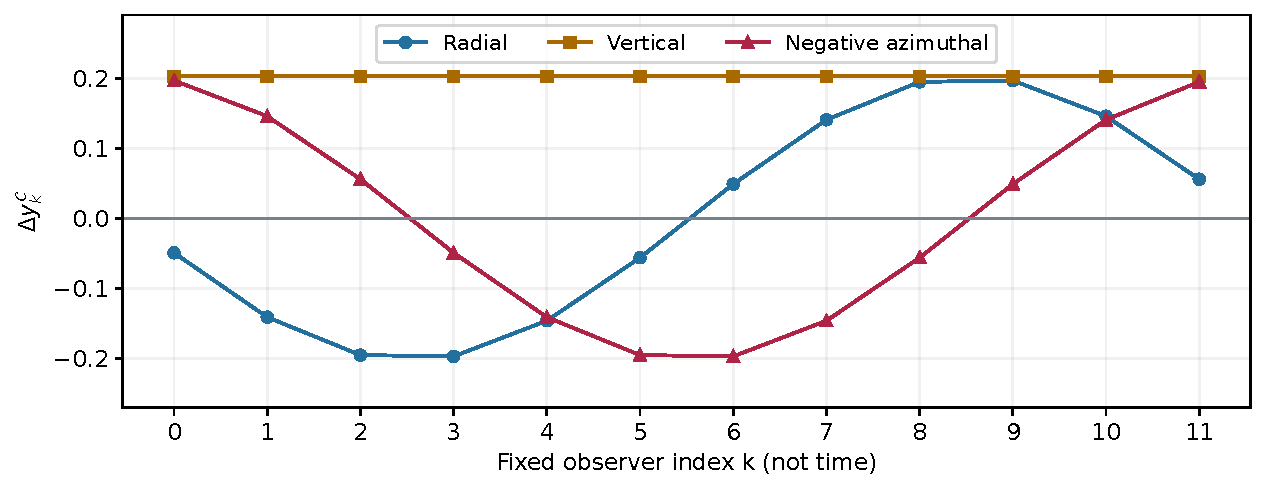
\includegraphics[width=\linewidth]{figures/state_contrast.pdf}
\caption{A fixed-state contrast from SRG-03: $(1,1,1)$ and $(1,e^{i\pi/6},1)$ have $I=3$, hence equal staged $z_s$ and $M$ at the common clock $(q,N,t_c)=(0,12,0)$. Chirality changes by $(-1/2,0,1/2)$. The plotted differences are $B_k\tr A\Delta\Ch$, using $A=aR_z(\pi/2-0.244)$ and $\phi_0=0$. They are fixed-site components with DC/first spatial harmonics, not successive native states or travelling data.}\label{fig:contrast}
\end{figure}

\section{A short cubic-information and subsystem comparison}\label{sec:cubic}
The historical handoff uses $J(\Omega)=\Im(\Omega_1\overline\Omega_2\Omega_3)$, which is not among the staged invariants. This limited comparison explains an information boundary without adopting a receiver model.

\begin{proposition}[Missing cubic data]\label{prop:cubic}
The complete uniform staged records, including every paired and circle-tangent projection, do not determine $J$. Consequently they do not determine the sourced historical parameter handoff from an arbitrary finite completed $J$ record.
\end{proposition}
\begin{proof}
Let $\Omega=(1,e^{i\pi/6},1)$ and $\Omega'=-\Omega$. Both have $I=3$ and $\Ch=(-1/2,0,1/2)$, so all staged records at a common clock coincide. But the cubic products are $e^{-i\pi/6}$ and $-e^{-i\pi/6}$, giving $J=-1/2$ and $J'=+1/2$. For a nonempty finite real record the handoff forms
\begin{equation}\label{eq:handoff}
\mathcal N=\frac{\operatorname{mean}|J|}{\max|J|},\quad
\mathcal S=\operatorname{sign}(\operatorname{mean}J_{\rm tail}),\quad
(\alpha_e,\mu_e,\gamma_e)=
(\alpha_0(0.3+0.7\mathcal N),\ 0.6+0.2\mathcal S,\ 0.1(1+\mathcal N)).
\end{equation}
The denominator is one for an all-zero record, and the tail is the last twenty entries only when there are more than twenty entries. In the two singleton records $\mathcal N=1$, but $\mu_e=0.4$ and $0.8$. Thus equal staged observations yield different handoff parameters. Missing or empty records have the separate fallback $(\alpha_0,0.6,0.2)$ and are not the all-zero case. Optional historical measurement noise is absent from this counterexample.~\cite{Historical,SRG03}
\end{proof}

One extra correctly aligned $J$ per retained row is sufficient to evaluate \eqref{eq:handoff}; the two final statistics plus a missing/empty flag suffice if only its final output is desired. A present value is not a history. This is a finite real, fixed-channel, fixed-phase convention: the old helper is not being given an unproved NaN/overflow contract. The already sourced EMA variant is a different observation family, so Proposition~\ref{prop:cubic} is not a theorem about every possible Z readout.

\subsection{The limited twelve-site comparison}
The recovered RSB array has indices in $\C^3\otimes\C^{12}\otimes\C^2$. One can conditionally assign its middle index to the twelve spatial sites, provided an origin/cut and internal basis are declared. Its internal channel and helicity labels are not thereby native faces, gap pairs or physical helicity. The periodic difference operator $(L_{12}f)_k=f_{k-1}+f_{k+1}-2f_k$ obeys
\begin{equation}\label{eq:laplacian}
L_{12}\mathbf1=0,\qquad
L_{12}\cos\phi=(\sqrt3-2)\cos\phi,\qquad
L_{12}\sin\phi=(\sqrt3-2)\sin\phi.
\end{equation}
Indeed substituting $e^{im\phi_k}$ gives multiplier $2\cos(2\pi m/12)-2$; set $m=0,\pm1$. This is algebraic compatibility of the observed spatial modes, not a continuum Laplacian with a recovered geometric radius factor. Site-independent linear channel/helicity maps preserve this support because they commute with the spatial Fourier decomposition.

The source contraction has a separate obstruction. It chooses the first index maximizing site intensity and, for active nonadaptive $0<\alpha_e\le1$, retains multiplier one there and $1-\alpha_e$ elsewhere. Constant nonzero site data are invariant under cyclic shifts, yet first-index tie selection gives a nonuniform output distinguished at site zero. Shifting this output changes it, whereas shifting the input does not. Thus the rule is not globally cyclic-equivariant on ties. Subsequent scalar normalization cannot remove the unequal multipliers. Zero contraction is a distinct case. This exact counterexample is sufficient for the site-assignment qualification; no rule is repaired or executed.~\cite{RSB,SRG03}

The historical caller selects parameters from a completed record before a separate receiver run. There is no recovered operator coupling \eqref{eq:uniform} continuously into that receiver, no assignment of its state to the local circle, and no return term to \eqref{eq:native}. The comparison retains the accepted information boundary rather than choosing an autonomous spectral subsystem as physical toroidal dynamics.

\section{The declared delay-only comparator}\label{sec:delay}
The uniform law answers an orientation question, but it cannot answer whether a higher or more distant observer records a source earlier. SRG-04 therefore declares a second mathematical interface. It uses the same contacts, normals and observer frames, with a prescribed readout history and Euclidean delays. The distances supply arguments of a signal; they are not paths constrained to the red circle or material rays passing through panels.

For one readout $v$, write $W(t)=Av(t)$ and suppose its values are given at every retarded time needed below. No interpolation of native samples is implicit. An interpolation would require a separately chosen map $n\mapsto t_n$ and rule between samples; the native iteration $n$, supplied readout clock $(q,N,t_c)$, and analysis time $t$ remain distinct. Use contact index $\eta=(j,\sigma)$ when it avoids confusing the six labels with the scalar $a$.

\begin{definition}[Six-contact unit-gain delay reconstruction]\label{def:delay}
For a declared $c_*>0$, let
\begin{equation}\label{eq:delaylaw}
\begin{aligned}
q_\eta(t)&=n_\eta\tr W(t),&
d_\eta(X)&=\norm{X-P_\eta},&\tau_\eta(X)&=d_\eta(X)/c_*,\\
F(X,t)&=G^{-1}\sum_\eta n_\eta q_\eta(t-\tau_\eta(X)),&
Y_{mk}(t)&=B_{mk}\tr F(c_{mk},t).
\end{aligned}
\end{equation}
Here $G$ is exactly \eqref{eq:patchgram}. The histories for $M$ and $\Ch$ are kept separate; $T$ is their fixed linear blend.
\end{definition}
This definition has unit path gains and no spreading, blocking, damping, refraction or backreaction. It is an explicitly conditional comparison law from SRG-04, not a native propagation equation.~\cite[Eqn.~(3)]{SRG04} It has no evolving shared field state whose value is sampled by all sensors. Constant, harmonic and onset inputs used here are prescribed signal controls, not native trajectories.

\begin{proposition}[Baseline and covariance]\label{prop:baseline}
For constant $W$, or when all delays are zero, $F=W$ and $Y_{mk}=B_{mk}\tr W$. Under a common Euclidean coordinate change $X'=UX+a_0$, $U$ orthogonal, transform positions likewise and $n'=Un$, $A'=UA$, $B'=UB$, $G'=UGU\tr$. Then $F'(X',t)=UF(X,t)$ and $Y'=Y$.
\end{proposition}
\begin{proof}
Without differential time arguments the reconstruction is $G^{-1}\sum n_\eta n_\eta\tr W=W$. Orthogonal transformations preserve distances. Also $(UGU\tr)^{-1}=UG^{-1}U\tr$, $q'_\eta=(Un_\eta)\tr UW=q_\eta$, and substitution gives $F'=UF$. Left multiplication by $(UB)\tr$ cancels $U$. This includes improper coordinate changes; keeping $G$ artificially diagonal after a general rotation would fail this proof.
\end{proof}

\begin{proposition}[Contact-onset half-value]\label{prop:half}
Let $W(t)=w_0\mathbf1_{t\ge0}$ with zero prehistory. At $X=P_\eta$, for $t>0$ smaller than every other contact's delay,
\begin{equation}\label{eq:half}
n_\eta\tr F(P_\eta,t)=\tfrac12 q_\eta(t).
\end{equation}
In particular, when $q_\eta\ne0$ the assigned source value is not an imposed Dirichlet value of the reconstructed field.
\end{proposition}
\begin{proof}
All six contacts are distinct, so the stated interval is nonempty. Only the zero-length self-channel has arrived. Its projected reconstruction is $(n_\eta\tr G^{-1}n_\eta)q_\eta$. From \eqref{eq:planes} and \eqref{eq:patchgram},
\[
n_\eta\tr G^{-1}n_\eta=\frac47\frac7{12}+\frac37\frac7{18}
=\frac13+\frac16=\frac12.
\]
Choose, for example, $w_0=n_\eta$ to obtain the nonzero discrepancy. This is a counterexample within the declared law, not an inconsistency requiring replacement of that law.
\end{proof}
One may evaluate $F$ on $\Gamma_j$ and project onto its tangent. At the two contacts these projections equal $-(n_j^+)\tr F$ and $(n_j^-)\tr F$ respectively, but generally not the original instantaneous $-q_j^+$ and $q_j^-$. The circle angle is still a spatial variable, not travel time.

\section{Transfer bounds and a controlled inverse}\label{sec:transfer}
For the formal harmonic input $W(t)=\Re(\widehat w e^{i\omega t})$, with real $\omega$, define
\begin{equation}\label{eq:transfer}
\mathbf K(X,\omega)=G^{-1}\sum_\eta n_\eta n_\eta\tr e^{-i\omega\tau_\eta(X)},
\qquad \widehat Y_{mk}=B_{mk}\tr\mathbf K(c_{mk},\omega)\widehat w.
\end{equation}
This is an exact substitution into \eqref{eq:delaylaw}, not numerical evolution. In particular $\mathbf K(X,0)=\Id_3$.

\begin{theorem}[Compression, remainder and low-frequency invertibility]\label{thm:compression}
At any fixed position with finite delays, let $V=N_\Delta G^{-1/2}$ and define
\[
\norm L_G:=\norm{G^{1/2}LG^{-1/2}}_2.
\]
Then $V^*V=\Id_3$ and
\begin{equation}\label{eq:compression}
G^{1/2}\mathbf K G^{-1/2}
=V^*\diag(e^{-i\omega\tau_\eta})V,\qquad \norm{\mathbf K}_G\le1.
\end{equation}
For a reference delay $\tau_0$, set $\delta_\eta=\tau_\eta-\tau_0$, $\Delta=\max_\eta|\delta_\eta|$ and
\[
D_\delta=G^{-1}\sum_\eta n_\eta n_\eta\tr\delta_\eta.
\]
There is an exact expansion
\begin{equation}\label{eq:taylor}
\mathbf K=e^{-i\omega\tau_0}(\Id_3-i\omega D_\delta+E_2),
\qquad \norm{E_2}_G\le\tfrac12\omega^2\Delta^2.
\end{equation}
Writing $s_{\min,G}$ for the minimum singular value of the conjugated operator,
\begin{equation}\label{eq:lowinverse}
s_{\min,G}(\mathbf K)\ge1-|\omega|\Delta.
\end{equation}
Thus $|\omega|\Delta<1$ suffices for invertibility. The midpoint $\tau_0=(\tau_{\max}+\tau_{\min})/2$ minimizes $\Delta$.
\end{theorem}
\begin{proof}
By the definition of $G$, $V^*V=G^{-1/2}N_\Delta\tr N_\Delta G^{-1/2}=\Id_3$. Direct multiplication yields \eqref{eq:compression}. The middle diagonal operator is unitary, and the isometry $V$ and its adjoint have norm one, proving the weighted contraction.

For real $x$, two integrations of the exponential derivative give
\[
e^{-ix}-1+ix=-x^2\int_0^1(1-u)e^{-iux}\,du,
\quad |e^{-ix}-1+ix|\le x^2/2.
\]
Apply this identity to each $x=\omega\delta_\eta$ and compress by $V^*,V$. The constant term becomes the identity, the linear term becomes $-i\omega G^{1/2}D_\delta G^{-1/2}$, and the diagonal remainder norm is at most $\omega^2\Delta^2/2$. Undoing the similarity gives \eqref{eq:taylor}. Notice also that $GD_\delta$ is real symmetric.

The first-order difference estimate $|e^{-ix}-1|\le|x|$, from one integration, gives
\[
\norm{e^{i\omega\tau_0}\mathbf K-\Id_3}_G\le|\omega|\Delta.
\]
For a unit vector $z$ in the conjugated coordinates, the reverse triangle inequality then gives a norm of its image at least $1-|\omega|\Delta$. Taking the infimum proves \eqref{eq:lowinverse}. Finally, any centre of the interval $[\tau_{\min},\tau_{\max}]$ has maximum distance to its endpoints at least half the interval length. The midpoint attains that value, proving its minimax property.
\end{proof}

The small quantity is differential phase $|\omega|\Delta$, not necessarily the common phase $|\omega\tau_0|$. If every delay is $\tau_0$, the law is exactly a common shift. In general the bound is in the $G$ norm; no unqualified Euclidean contraction or physical energy monotonicity follows. Even a bounded invertible transfer at each frequency does not by itself produce a causal, stable real-time inverse.

\section{Height, radius, symmetry and reception}\label{sec:timing}
\subsection{Distance derivatives and an earliest possible onset}
Let $X-O=R e_r(\phi)+h\ez$, and $\gamma_j=\pi/2+2\pi j/3$. Subtracting the contact coordinates gives
\begin{equation}\label{eq:distance}
d_{j\sigma}^2=R^2+a^2-2aR\cos(\phi-\gamma_j)+(h-\sigma a)^2.
\end{equation}
Away from $d_{j\sigma}=0$, differentiation yields
\begin{equation}\label{eq:derivatives}
\partial_h d_{j\sigma}=\frac{h-\sigma a}{d_{j\sigma}},\qquad
\partial_R d_{j\sigma}=\frac{R-a\cos(\phi-\gamma_j)}{d_{j\sigma}}.
\end{equation}
At fixed $R,\phi$, moving from height zero toward $a$ shortens each upper-contact distance and lengthens each lower-contact distance. Above $a$, both sets increase. If $R>a$, all six distances increase with radius. Without this hypothesis, horizontal motion toward a contact can shorten a distance, so there is no universal radius statement. Changing height and radius together would mix these effects; this is the reason for the separated controls.

\begin{proposition}[Onset and its detection qualification]\label{prop:onset}
For simultaneous causal contact inputs with zero prehistory, the geometrically earliest possible delay is
\begin{equation}\label{eq:onset}
\tau_{\min}(R,\phi,h)=\frac1{c_*}\sqrt{R^2+a^2-2aR\max_j\cos(\phi-\gamma_j)+(|h|-a)^2}.
\end{equation}
For a step input $W=w_0\mathbf1_{t\ge0}$, let $\mathcal A$ be the group of earliest tied contacts. Its full-vector contribution is zero exactly when $n_\eta\tr w_0=0$ for every $\eta\in\mathcal A$. An individual observed component can vanish even if the full vector is nonzero.
\end{proposition}
\begin{proof}
Minimizing \eqref{eq:distance} over $j$ selects the maximum cosine, and minimizing over the independent sign selects $(|h|-a)^2$. No channel can arrive earlier under the stipulated zero prehistory. Put $Q_{\mathcal A}:=\sum_{\eta\in\mathcal A}n_\eta n_\eta\tr$. The first step contribution is $G^{-1}Q_{\mathcal A}w_0$. Since $G$ is invertible, it vanishes iff $Q_{\mathcal A}w_0=0$. The quadratic form is
\[
w_0\tr Q_{\mathcal A}w_0=\sum_{\eta\in\mathcal A}(n_\eta\tr w_0)^2.
\]
Its vanishing is equivalent to every summand vanishing, proving the full-vector claim. A projection onto one frame vector can annihilate a nonzero vector, establishing the component qualification.
\end{proof}

At an aligned site $\phi=\gamma_0$, $c_*\tau_{\min}=\sqrt{(R-a)^2+(|h|-a)^2}$. For $R=3$, the H levels $h=\pm a$ have distance $2.594480\ldots$, while $h=0,\pm2a$ all have distance $2.625981\ldots$. The higher outer levels therefore lose the earlier-arrival advantage in this height-only comparison. The values do not promise a nonzero signal for every source, and an eternal harmonic has phases without a first-arrival time.

\subsection{Reflection and threefold covariance}
\begin{proposition}[Exact parity relations]\label{prop:parity}
For $S_z=\diag(1,1,-1)$,
\begin{equation}\label{eq:parity}
\mathbf K(R,\phi,-h;\omega)=S_z\mathbf K(R,\phi,h;\omega)S_z.
\end{equation}
If $S_z\widehat w=p\widehat w$, $p\in\{+1,-1\}$, the matched same-frame records obey
\[
\widehat Y_- =p\diag(1,-1,1)\widehat Y_+.
\]
For the rotation $Q=R_z(2\pi/3)$ about $O$,
\begin{equation}\label{eq:c3}
\mathbf K(O+Q(X-O),\omega)=Q\mathbf K(X,\omega)Q\tr.
\end{equation}
\end{proposition}
\begin{proof}
Reflection interchanges $P_j^+$ with $P_j^-$ and $n_j^+$ with $n_j^-$. Thus delays are permuted and the dyads transform by $S_z$. The diagonal $G$ commutes with $S_z$, giving \eqref{eq:parity}. It follows that $\widehat F_-=pS_z\widehat F_+$. From \eqref{eq:frames}, $B\tr S_z B=\diag(1,-1,1)$, which gives the local-frame relation. Horizontal source vectors have $p=+1$ and vertical vectors have $p=-1$; a general vector is the sum of its two parity parts. For $Q$, the same proof uses the cyclic permutation $j\mapsto j+1$, $n\mapsto Qn$, and $QG=GQ$.
\end{proof}
At $h=0$, \eqref{eq:parity} rules out horizontal/vertical off-block mixing. At angular indices separated by four sites, \eqref{eq:c3} gives identical local records for a vertical source; a general fixed source must be rotated correspondingly before identical records follow. These response symmetries do not repair the body-reflection failure of Proposition~\ref{prop:mirror}; they are statements about the declared frames and input law.

\section{A pure-delay component and a blind-frequency counterexample}\label{sec:aligned}
An aligned equatorial position separates signal delay from amplitude interference particularly clearly. Let $R>0$, $h=0$, $\phi=\gamma_0$. The two contacts of pair zero have distance $d_0$, and the other four have distance $d_1$, where
\begin{equation}\label{eq:twodist}
d_0=\sqrt{(R-a)^2+a^2},\quad
d_1=\sqrt{R^2+aR+2a^2},\quad e_i=e^{-i\omega d_i/c_*}.
\end{equation}

\begin{theorem}[Aligned decomposition and all-frequency inverse]\label{thm:aligned}
In the common orthonormal basis $(u_0,v_0,\ez)$,
\begin{equation}\label{eq:aligned}
\mathbf K=\diag\left(\frac{2e_0+e_1}{3},\ e_1,\ \frac{e_0+2e_1}{3}\right).
\end{equation}
The tangential component is exactly a unit-gain delay $d_1/c_*$. For every real $\omega$, this site is invertible with Euclidean minimum singular value at least $1/3$. Consequently every accepted equatorial R ring, which contains an aligned site and records all three frame components, has a stacked transfer of rank exactly three at every real frequency.
\end{theorem}
\begin{proof}
Pair zero contributes the dyad $(8/7)u_0u_0\tr+(6/7)\ez\ez\tr$ with phase $e_0$. The remaining two pairs have $\sum_{j=1,2}u_ju_j\tr=(1/2)u_0u_0\tr+(3/2)v_0v_0\tr$, so their sum contributes $(4/7)u_0u_0\tr+(12/7)v_0v_0\tr+(12/7)\ez\ez\tr$ with phase $e_1$. Multiplication by $G^{-1}$ gives \eqref{eq:aligned}. In particular $v_0$ is orthogonal to both nearest normals; its source signal cannot arrive through the nearer pair.

Since $|e_i|=1$, the reverse triangle inequality gives $|2e_0+e_1|\ge1$ and $|e_0+2e_1|\ge1$. The diagonal basis is orthonormal, so these bounds divided by three and $|e_1|=1$ are exactly the singular-value lower bounds. A full local frame is orthogonal and preserves invertibility. A stack containing this invertible three-row block has rank at least three and, because it maps a single $\C^3$ source, at most three.
\end{proof}

The radial and vertical gains have equal squared magnitude,
\begin{equation}\label{eq:gain}
|\mathbf K_{zz}|^2=\frac{5+4\cos[\omega(d_1-d_0)/c_*]}9\in[1/9,1].
\end{equation}
This follows by multiplying the corresponding phasor sum by its conjugate. Distance is not required to weaken the signal in a unit-gain law. The tangential delay increases with radius because $d_1'=(R+a/2)/d_1>0$, while its magnitude remains one. The vertical magnitude changes with differential phase, not a spreading factor.

\begin{table}[htbp]\centering
\caption{Accepted aligned R fixtures. Distances are in shell-width units; gain uses the one prescribed phase condition $\omega a/c_*=\pi/2$. Rounded entries are manuscript-local substitutions, not a parameter scan.}
\begin{tabular}{@{}rrrr@{}}\toprule
$R$ & $d_0$ & $d_1$ & $|\mathbf K_{zz}|^2$\\\midrule
2 & 1.645240 & 2.267142 & 0.225148\\
3 & 2.625981 & 3.247376 & 0.225732\\
4 & 3.617283 & 4.236859 & 0.227840\\\bottomrule
\end{tabular}\label{tab:radius}
\end{table}

\begin{proposition}[Off-ring axial blindness]\label{prop:axis}
At $X=O+h\ez$, with no admissible positive-radius observer ring implied, let
\[
d_\pm=\sqrt{a^2+(h\mp a)^2},\qquad \tau_\pm=d_\pm/c_*.
\]
Then
\begin{equation}\label{eq:axis}
\mathbf K_{\rm axis}=e^{-i\omega(\tau_++\tau_-)/2}
\cos\!\left(\frac{\omega(\tau_+-\tau_-)}2\right)\Id_3.
\end{equation}
At $h=0$ it is a common shift. At $h\ne0$ it vanishes at each odd-$\pi$ differential phase.
\end{proposition}
\begin{proof}
For either sign, $\sum_j n_j^\sigma(n_j^\sigma)\tr=G/2$: the mixed terms cancel because $\sum u_j=0$, and the horizontal and vertical terms each make half the full Gram matrix. Thus $\mathbf K=(e^{-i\omega\tau_+}+e^{-i\omega\tau_-})\Id_3/2$, which is \eqref{eq:axis}. The squared-distance difference is $-4ha$, so for $h\ne0$ the two delays differ. Choosing $\omega(\tau_+-\tau_-)=(2m+1)\pi$ gives zero. This diagnostic lies at $R=0$, outside the $R_m>0$ ring family.
\end{proof}

\begin{figure}[htbp]\centering
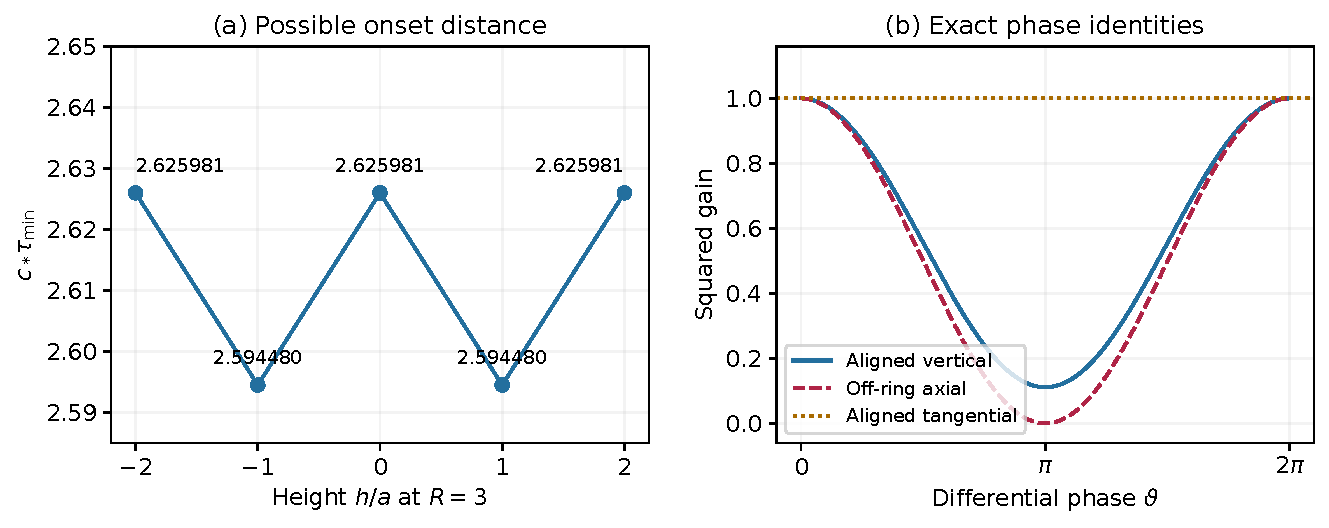
\includegraphics[width=\linewidth]{figures/delay_comparison.pdf}
\caption{Static reception comparison. Left: the accepted five-height nearest-distance values at the aligned $R=3$ site, divided by the symbolic $c_*$ to obtain possible arrival times. Right: analytic phase identities, with $\vartheta$ denoting differential phase. At aligned equatorial sites the squared vertical gain is $(5+4\cos\vartheta)/9$ and never vanishes; the tangential gain is one. At an off-ring axial point it is $\cos^2(\vartheta/2)$ and is zero at $\vartheta=\pi$. Curves sample closed formulas for drawing only; they are not time evolutions or a new frequency experiment.}\label{fig:delay}
\end{figure}

Theorem~\ref{thm:aligned} is therefore an aligned-site result, not a theorem for every point or every H family. Its validity depends on full-frame records; a scalar-only channel may still miss source components.

\section{Information and calibration in the delayed records}\label{sec:information}
At a fixed frequency, stack any finite collection of full-frame outputs for one source $\widehat w$. Every row factors through that same $\widehat w\in\C^3$, so the complex signal rank is at most three. The aligned R theorem supplies equality for those arrays. Additional sites can constrain a proposed transfer law, provide redundancy, or avoid a bad location without creating new coordinates of that source. The separate $M$ and $\Ch$ signals remain subject to their native/readout definitions; $T$ adds no independent input under a known blend.

A simultaneous delayed measurement depends on a history. It cannot inherit the instantaneous rank-four theorem by merely counting its outputs. If two prescribed state/readout histories have the same $I$ and $\Ch$ at every retarded argument and use the same supplied clock, their staged histories and all records of \eqref{eq:delaylaw} agree, by pointwise substitution. Pointwise common-phase changes leave those quantities unchanged while generally changing $J$. Whether both prescribed histories are trajectories of \eqref{eq:native}--\eqref{eq:sync} is a separate dynamical question, not established here. This is an exact statement about the observation operator, with no claim of native trajectory observability.

For a known nonzero tangential harmonic at two aligned equatorial sites, the ratio in the common $v_0$ component is
\begin{equation}\label{eq:aliases}
\frac{\widehat Y_2^{\rm tan}}{\widehat Y_1^{\rm tan}}
=\exp\!\left(-i\omega\frac{d_1(R_2)-d_1(R_1)}{c_*}\right).
\end{equation}
The common source phase cancels, but a single nonzero frequency determines reciprocal speed only modulo $2\pi/(\omega\Delta d_1)$, subject to positive-speed admissibility. This follows because adding that increment to $1/c_*$ changes the exponent by an integer multiple of $2\pi i$. Unknown site-clock offsets can produce the same phase difference. An unknown absolute length unit confounds length with speed; unknown frame or channel gains can confound extraction of the tangential component. Constant signals provide no speed information at all. Further frequencies or sites may constrain aliases, but uniqueness needs stated calibration and an admissible interval or phase-unwrapping condition. No speed is fitted here.

\section{An auxiliary delay-line storage balance}\label{sec:storage}
An ideal delay channel has a useful realization, provided its added state and initialization are named. For a real scalar input $q$, a length $d>0$ and the same $c_*>0$, take
\begin{equation}\label{eq:transport}
u_t+c_*u_\xi=0,\quad 0<\xi<d,\qquad u(0,t)=q(t).
\end{equation}
This one-way transport model is auxiliary to the signal law, not the shared periodic carrier considered in Paper II. Its coordinate $\xi$ is a line coordinate, not distance along $\Gamma_j$.

\begin{theorem}[Characteristics and model-defined storage]\label{thm:storage}
For $C^1$ input and compatible prehistory $u(\xi,0)=q(-\xi/c_*)$, the solution is $u(\xi,t)=q(t-\xi/c_*)$. The quadratic storage and its boundary balance are
\begin{equation}\label{eq:storage}
\begin{aligned}
E(t)&=\frac12\int_0^d u(\xi,t)^2\,d\xi
=\frac{c_*}{2}\int_{t-d/c_*}^{t}q(r)^2\,dr,\\
\dot E(t)&=\frac{c_*}{2}\big[q(t)^2-q(t-d/c_*)^2\big].
\end{aligned}
\end{equation}
For piecewise $C^1$ initial data $u_0$ with $u_0(0)=q(0)$, the characteristic solution before reaching the inlet is $u_0(\xi-c_*t)$, and after that it is $q(t-\xi/c_*)$. The boundary balance remains $\dot E=(c_*/2)[u(0,t)^2-u(d,t)^2]$ wherever the classical derivatives exist, and almost everywhere for the piecewise smooth solution. The delayed-input expression for the outlet holds only after the initial contents have left.
\end{theorem}
\begin{proof}
Along a line $\xi-c_*t=\text{constant}$, differentiation gives $d u/dt=u_t+c_*u_\xi=0$. Tracing backwards reaches either $(\xi-c_*t,0)$ or $(0,t-\xi/c_*)$, proving both characteristic formulas. For pure-delay prehistory they coincide. Substitution $r=t-\xi/c_*$ gives the second integral in \eqref{eq:storage}, and the fundamental theorem of calculus gives its derivative. Independently, multiplying \eqref{eq:transport} by $u$ and integrating yields
\[
\dot E=-c_*\int_0^d u u_\xi\,d\xi
=\frac{c_*}{2}[u(0,t)^2-u(d,t)^2],
\]
which also proves the arbitrary-initial-data balance. Piecewise smooth inputs, including a step with zero prehistory, are interpreted along characteristics; the integral balance remains valid and its derivative holds almost everywhere. At $d=0$ there is an immediate identity channel and zero storage.
\end{proof}

For a sustained real harmonic $q(t)=\Re(\widehat q e^{i\omega t})$, $\omega\ne0$, averaging $q^2$ over one period gives $|\widehat q|^2/2$. Thus mean storage is $d|\widehat q|^2/4$ and the two mean boundary rates are both $c_*|\widehat q|^2/4$. For constant real $q_0$, they instead are $dq_0^2/2$ and $c_*q_0^2/2$. These follow directly from \eqref{eq:storage}; no time integration is required.

The units are signal squared times length, with rates per analysis-time unit. Nothing identifies $E$ with a native Hamiltonian or physical energy emitted by the core. There is a decisive duplication limitation: adding an independent copy of the same delay channel leaves $q$ unchanged and adds another identical storage and boundary-rate term. Arbitrarily many independent sensor paths can therefore multiply the sum without debiting a shared source. The reconstruction weights in $F$ do not provide that debit. A shared-carrier model needs its own state, allocation or input operator, geometry and balance; closed reciprocal exchange would require backreaction as well. A one-way delay does not establish a returning or circulating path.

\section{Conclusions and the boundary of the series}\label{sec:conclusions}
The author's paired upper/lower picture admits a precise conditional realization. With the median contacts fixed and normal crossing required, a unique circle in the selected median plane has a centre and radius determined by the patch geometry. Its contacts lie inside finite triangles, and the entire circle avoids the material panels. The six contacts cannot belong to one planar circle; three symmetry-related local circles are possible and mutually disjoint. The material object remains the inherited annulus. None of these statements fixes a physical loop count or tube thickness.

The complete quarter-turned observer placement has an explicit centre, pivot convention, frame, scale and translation. Full-panel clearance follows from enclosing balls. The H and R comparisons distinguish height from radius, retain 84 distinct sites among 96 labels, and expose the difference between mirrored centres and mirrored bodies. Their placement rings and the local circles remain separate geometries.

Under the first observation law, complete frames reconstruct a registered vector, but repetition adds no noiseless source dimension. For fixed known staged calibration the generic native information is $(I,\Ch)$, with real rank four and explicit invisible directions, singular strata and inversion limits. The cubic counterexample identifies data that those records omit. A conditional twelve-site spectral assignment does not eliminate that omission or the source contraction's tie preference.

Under the second law, declared delays recover the uniform baseline when they vanish. They supply exact timing and parity comparisons, a weighted transfer bound, and an aligned pure-delay component whose gain is independent of distance. Unequal phasor weights give an all-frequency inverse at aligned equatorial sites; equal axial weights permit complete blind frequencies elsewhere. The contact half-value and independent-channel storage calculation specify the model's limitations without invalidating its internal mathematics.

Subsequent papers address an explicitly driven shared carrier and exterior reception, followed by compact encodings, collisions and nonlinear saturation. Those models are distinct from the conditional geometric and observation maps established here. What remains open here is the adoption of a physical channel-to-space dictionary, a shared material connection, calibrated source work and reciprocal coupling. Those choices are not prerequisites for the geometric and observation theorems just proved.

\section*{Acknowledgements}
\addcontentsline{toc}{section}{Acknowledgements}
Hilmir Fr\'imann Halld\'orsson originated and directed the paired-gap, transverse-loop, twelve-module and multi-ring questions developed here. The work forms part of a sustained human--AI collaboration, including earlier exploration with GPT-4o, GPT-assisted formulation and internal mathematical review, and Codex-assisted source recovery, derivation, checks, figure preparation and typesetting. The internal reviews are not external peer review.

\appendix
\section{Exact coordinates and a reproducibility dictionary}\label{app:coords}
The panel maps \eqref{eq:panels}, local vertices \eqref{eq:octagon} and welded cycles in Section~\ref{sec:shell} define all coordinates without software. For direct reference, the eighteen global vertices are listed below. The notation $h_0=(\sqrt2-1)/2$ shortens the six seam endpoints. The ordering matches Paper C and the retained coordinate data.
\begin{center}\small
\begin{tabular}{@{}rccc@{}}\toprule
ID & $x$ & $y$ & $z$\\\midrule
0 & $0$ & $\sqrt3/2$ & $-h_0$\\
1 & $-1/2+\sqrt2/4$ & $\sqrt6/4$ & $-1/2$\\
2 & $-\sqrt2/4$ & $\sqrt3/2-\sqrt6/4$ & $-1/2$\\
3 & $-1/2$ & $0$ & $-h_0$\\
4 & $-1/2$ & $0$ & $h_0$\\
5 & $-\sqrt2/4$ & $\sqrt3/2-\sqrt6/4$ & $1/2$\\
6 & $-1/2+\sqrt2/4$ & $\sqrt6/4$ & $1/2$\\
7 & $0$ & $\sqrt3/2$ & $h_0$\\
8 & $-h_0$ & $0$ & $-1/2$\\
9 & $h_0$ & $0$ & $-1/2$\\
10 & $1/2$ & $0$ & $-h_0$\\
11 & $1/2$ & $0$ & $h_0$\\
12 & $h_0$ & $0$ & $1/2$\\
13 & $-h_0$ & $0$ & $1/2$\\
14 & $\sqrt2/4$ & $\sqrt3/2-\sqrt6/4$ & $-1/2$\\
15 & $1/2-\sqrt2/4$ & $\sqrt6/4$ & $-1/2$\\
16 & $1/2-\sqrt2/4$ & $\sqrt6/4$ & $1/2$\\
17 & $\sqrt2/4$ & $\sqrt3/2-\sqrt6/4$ & $1/2$\\\bottomrule
\end{tabular}
\end{center}
The three face cycles are $(0,1,2,3,4,5,6,7)$, $(3,8,9,10,11,12,13,4)$ and $(10,14,15,0,7,16,17,11)$. Each consecutive pair, including closure, is a material edge; the three shared pairs are counted only once. The measurement bases in Section~\ref{sec:shell} are not appended to these cycles.

The coordinate formulas above, together with the stated panel cycles, give a complete geometric specification. The accompanying source map identifies the retained coordinate data and the definitions used for each construction.

\section{Manuscript-local verification and figure construction}\label{app:checks}
The mathematical arguments in the main text establish the all-parameter statements. The manuscript checks verify displayed algebraic identities, rational inequality certificates, the fixed tables and the coordinates used in this edition. The static figure renderer uses retained coordinates, frames and selected state-contrast data. Circle and analytic phase samples are drawing primitives, not time steps or native trajectories.

The figure presentation separates solid material edges, dashed measurement closures, conditional local curves and reference axes. Figures~\ref{fig:geometry}--\ref{fig:delay} use the retained data, with presentation choices limited to camera, typography and panel layout. No new observer position, carrier or finite tube thickness is selected.

Finite checks support the transcription of the displayed formulas and data; the proofs establish their stated domains of validity. Counterexamples and exceptional cases delimit those domains.

\begin{thebibliography}{99}\raggedright
\bibitem{PC} H. Fr\'imann Halld\'orsson. \emph{Exact Geometry of the Folded Tri-Octagon Module}. Paper C, publication revision v1.0.1, 23 September 2026. Sections 2--5, especially Theorems 1 and 1b in Section 5.
\bibitem{Origins} H. Fr\'imann Halld\'orsson. \emph{Tri-Octagon: Geometric Origins, Normalization, and Constant Interpretations}. GEO-ORIGINS-01, v0.1, 17 October 2026. Sections 1--4.
\bibitem{AuthorPair} H. Fr\'imann Halld\'orsson. Unpublished design notes on paired upper/lower regions and a transverse loop (author clarification), 18 October 2026. Private source record.
\bibitem{AuthorScope} H. Fr\'imann Halld\'orsson. \emph{Author scope}. Unpublished clarification of native-state, local-loop and twelve-observer questions, 18 October 2026. Private source record.
\bibitem{AuthorMulti} H. Fr\'imann Halld\'orsson. \emph{Author multi-ring proposal}. Unpublished higher/lower and outward-array design notes, 18 October 2026. Private source record.
\bibitem{Gate} Codex research record. \emph{Gate/Torus Investigation}, v0.1, REPORT. Sections 2--3 and 6: finite regions, conditional contact family and complete quarter-turned motif. Unpublished source snapshot retained in SRG-02, 18 October 2026.
\bibitem{GateDirections} Codex research record. \emph{Direction Invariants Report}. Gate/Torus continuation, Section 5: contact qualifications. Unpublished source snapshot retained in SRG-02, 18 October 2026.
\bibitem{Native} \emph{Native Tri-Octagon source definitions}: \texttt{DYNAMICS.py}, \texttt{GEOMETRY.py}, \texttt{FACE\_STATE.py}, \texttt{READOUTS.py}. Source snapshots retained in SRG-02--03, 18 October 2026. Recurrence, face encoding, coordinates and raw channel chirality.
\bibitem{Readout} \emph{Z manifold source definitions}: \texttt{Z\_MANIFOLD.py}. Source snapshot retained in SRG-02--03, 18 October 2026. Clock, staged configuration, scalar, macro and blend definitions, lines 47--199. The scalar is denoted $z_s$ here.
\bibitem{SRG02} Codex, with Hilmir Fr\'imann Halld\'orsson's geometric direction. \emph{Paired Gap Geometry and Transverse Toroid Comparison}. SRG-PAIRED-GAP-TOROID-02, 18 October 2026. Unpublished research report, equations (1)--(5), coordinate data and source registry.
\bibitem{SRG03} Codex, with Hilmir Fr\'imann Halld\'orsson's direction. \emph{Native Response at Twelve Toroidal Observers}. SRG-TOROID-RESPONSE-03, 18 October 2026. Unpublished research report, equations (1)--(15), observer map and source registry.
\bibitem{SRG04} Codex, with Hilmir Fr\'imann Halld\'orsson's multi-ring question. \emph{SRG-SPATIAL-RESPONSE-04---what multiple rings can test}. 18 October 2026. Unpublished research report, equations (1)--(20), spatial map and source/adoption map.
\bibitem{Reviews} GPT. \emph{SRG-PAIRED-GAP-TOROID-02 review and question realignment}; \emph{SRG-TOROID-RESPONSE-03 mathematical review}; \emph{SRG-SPATIAL-RESPONSE-04 mathematical review}. 18 October 2026. Unpublished internal reviews with stated scope.
\bibitem{Historical} \emph{Historical cubic and parameter-selection sources}: \texttt{OLD\_DEFINITIONS.py}, \texttt{OLD\_SAMPLER.py}, and the relevant caller in \texttt{OLD\_TOY\_DISPLAY.py}. Source snapshots retained in SRG-02, 18 October 2026. Cubic expression and finite completed-record handoff.
\bibitem{RSB} \emph{Recovered RSB source}: \texttt{OLD\_RSB.py}. Source snapshot retained in SRG-02--03, 18 October 2026. Periodic phase operator and active phase-site contraction, especially lines 204--352. Conditional site assignment and tie counterexample in SRG-03.
\end{thebibliography}

\end{document}
